% ICML 2027 Two-Column Double-Blind Submission Draft
% Swap preamble to `\usepackage{icml2027}` once the official ICML 2027 style kit opens on Jan 8, 2027.
\documentclass[10pt,twocolumn]{article}
\usepackage[letterpaper,top=0.85in,bottom=0.85in,left=0.68in,right=0.68in,columnsep=0.25in]{geometry}
\usepackage[T1]{fontenc}
\usepackage{times}
\usepackage{natbib}
\setcitestyle{authoryear,round,citesep={;},aysep={,},yysep={;}}
\usepackage{fancyhdr}
\pagestyle{fancy}
\fancyhf{}
\lhead{\small\itshape Double-Blind Submission Draft (ICML 2027 Two-Column Format)}
\cfoot{\thepage}
\usepackage{amsmath,amssymb,amsthm,mathtools}
\usepackage{booktabs}
\usepackage{graphicx}
\usepackage{microtype}
\usepackage{xcolor}
\usepackage{enumitem}
\usepackage{url}
\usepackage[hidelinks]{hyperref}

\newtheorem{theorem}{Theorem}
\newtheorem{proposition}{Proposition}
\newtheorem{remark}{Remark}

\setlist[itemize]{leftmargin=1.4em,itemsep=2pt,topsep=3pt}
\newcommand{\KL}{D_{\mathrm{KL}}}

\title{\Large\bfseries Steerable Before Decodable: Multi-Model Causal Evidence of Unembedding-Orthogonal Bottlenecks Beyond the Logit and Tuned Lens}
\author{Anonymous Authors \\ \textit{Paper under double-blind review}}
\date{}
\begin{document}
\maketitle
\begin{abstract}
Interpretability pipelines routinely assume that if a transformer represents a concept linearly in its residual stream, that concept can be decoded by projecting intermediate activations through the unembedding matrix (Logit Lens) or a trained affine translator (Tuned Lens). Evaluating 4 distinct open-weight model families spanning 1.7B to 7.3B parameters (Qwen3-1.7B, SmolLM2-1.7B, Mistral-7B, OLMo-2-7B) across 4 real-world comparative domains and 2,688 strictly held-out cross-lexicon entity pairs (100\% single-token across all 4 tokenizers), we test this assumption against gradient-weighted Paired-Swap Algorithmic Core Extraction (ACE) and six strong baselines---including an exact \textbf{KL-Minimizing General-Corpus Tuned Lens} (Belrose et al.\ 2023 KL objective on 3,600 scientific tokens), Ridge General-Corpus Tuned Lens, Domain Tuned Lens, Direct Logit Lens, Contrastive Activation Addition (CAA), and $L_2$ Logistic Probes. Across 16 (model, domain) cells, peak 1D causal steering emerges where ACE linear readout (mean AUC 0.765) significantly outperforms KL-Minimizing General-Corpus Tuned Lens (0.638, gap +0.127, Wilcoxon $p=0.0107$), Ridge General Tuned Lens (0.693, $p=0.0370$), Domain Tuned Lens (0.708, $p=0.0467$), and Direct Logit Lens (0.727), while operating largely orthogonal to $\Delta W_U$ (mean $|\cos(q_{\ell^*}, \Delta W_U)| = 0.140$). On 1D causal necessity (Flip-1D), ACE achieves mean cross-lexicon reversal +0.235---outperforming random controls (-0.0009, $p=1.53e-05$), CAA (+0.170, $p=1.53e-04$), and $L_2$ Probes (+0.179, $p=3.81e-03$). On 1D sufficiency (Keep-1D), deleting 2,047--4,095 orthogonal dimensions outperforms the unperturbed model in 16/16 cells (sign-test $p=1.53e-05$; 0.799 vs.\ 0.712 clean). In multi-token generation, sustaining Flip-1D at every decode step boosts causal reversal up to 8$\times$ (5.6\% to 44.4\% on Qwen3-1.7B \texttt{physical\_scale}; 0.0\% to 20.0\% on SmolLM2-1.7B \texttt{hazard\_severity}, vs.\ 0.0\% sustained random) with fluent NLL, directly confirming KV-cache re-attention. Finally, on a non-comparative natural-language benchmark of real disjoint scientific abstracts ($n=60$ held-out papers), Qwen3-1.7B exhibits ACE readout 0.979 vs.\ KL-Tuned Lens 0.546 at $|\cos|=0.017$, and Keep-1D rescues clean AUC from 0.548 to 0.922 (+0.374).
\end{abstract}


\section{Introduction}
Vocabulary-projection lenses---the Direct Logit Lens \citep{nostalgebraist2020logitlens} and the learned affine Tuned Lens \citep{belrose2023tunedlens}---are standard diagnostic instruments for inspecting how transformer layers assemble predictions. However, recent evidence on function vectors \citep{todd2024function,steerable2026} suggests a geometric dissociation: linear steering directions can control downstream model behavior at intermediate layers where unembedding projection decodes near chance.

We test whether this \emph{steerable-before-decodable} dissociation persists across four distinct open-weight architecture families (1.7B--7.3B: Qwen3-1.7B, SmolLM2-1.7B, Mistral-7B-v0.1, OLMo-2-1124-7B), survives both General-Corpus and Domain-Trained Residual-Affine Tuned Lenses, and extends to both 1D causal necessity (Flip-1D) and 1D causal sufficiency (Keep-1D) over 2,688 strictly held-out cross-lexicon entity pairs. Our findings establish four core results: (1) ACE readout (0.765) significantly exceeds both General-Corpus Tuned Lens (0.693, $p=0.037$) and Domain Tuned Lens (0.708, $p=0.047$) while remaining largely orthogonal to $\Delta W_U$ ($|\cos| = 0.140$); (2) gradient-weighted ACE Flip-1D (+0.235) significantly outperforms CAA \citep{panickssery2024caa}, $L_2$ probes \citep{alain2017probes}, and random controls; (3) Keep-1D rescues late-layer readout collapse in \textbf{16/16 cells} ($p=1.53e-05$, mean gain +0.087); and (4) single-position prefill steering preserves fluency but does not override KV-cache re-attention during unconstrained base-model multi-token generation.

\section{Related Work}
Early-decoding methods project intermediate residual states through $W_U$ directly \citep{nostalgebraist2020logitlens} or via layerwise affine translators \citep{belrose2023tunedlens}. Linear probing \citep{alain2017probes}, geometry-of-truth studies \citep{marks2024truth}, activation steering \citep{turner2023actadd,panickssery2024caa}, function vectors \citep{todd2024function}, distributed alignment search \citep{geiger2024das}, and transformer circuit analysis \citep{elhage2021circuits} study linear causal mediators. Motivated by \citet{steerable2026}, we provide the first 4-architecture, dual-Tuned-Lens, zero-leakage cross-lexicon audit comparing gradient-weighted Paired-Swap ACE against CAA and $L_2$ probes under both Flip-1D and Keep-1D.

\section{Methodology and Geometric Analysis}
Given ordered training entities $\{(e_i, y_i)\}$ and a source template $T_{\mathrm{src}}(A,B)$ with single-token contrast targets $(w^+, w^-)$, every unordered pair $\{i,j\}$ forms a symmetric swap pair $(x_{ij}, x_{ji})$ whose difference $\Delta h_\ell = h_\ell(x_{ij}) - h_\ell(x_{ji})$ cancels entity-order-invariant context. Letting $g_\ell = \partial(z_{w^+} - z_{w^-})/\partial h_\ell$ be the exact margin gradient backpropagated to layer $\ell$, Paired-Swap ACE extracts the top-$k$ orthonormal basis $Q_\ell \in \mathbb{R}^{D\times k}$ coupling swap covariance with downstream causal sensitivity:
\begin{align}
  A_\ell &= \tfrac{1}{P}\sum_{(a,b)} (h_{\ell,a} - h_{\ell,b})(h_{\ell,a} - h_{\ell,b})^\top + \varepsilon I, \nonumber \\
  M_\ell &= A_\ell^{1/2} G_\ell^\top / \sqrt{N}, \nonumber \\
  q_\ell &= \operatorname{normalize}\!\big(A_\ell^{1/2} u_1(M_\ell)\big), \label{eq:ace_cov} \\
  \operatorname{Flip\text{-}1D}(h) &= h - 2\langle h - \mu_\ell, q_\ell\rangle q_\ell, \label{eq:ace_flip} \\
  \operatorname{Keep\text{-}1D}(h) &= \mu_\ell + \langle h - \mu_\ell, q_\ell\rangle q_\ell, \nonumber \\
  \Delta_{\mathrm{flip}} &= \mathrm{AUC}_0 - \mathrm{AUC}_{\mathrm{flip}}. \label{eq:ace_keep}
\end{align}

\begin{theorem}[Unembedding-Orthogonality SNR Ceiling and Keep-1D Interference Cancellation]
Decompose the layer-$\ell$ residual state as $h_\ell = \mu_\ell + \alpha q_\ell + h_\perp$ with $h_\perp \perp q_\ell$, and let $u = \Delta W_U / \|\Delta W_U\|_2$ be the unit unembedding contrast direction.
(i) Under Direct Logit Lens projection onto $u$, the signal-to-interference ratio satisfies
\begin{equation}
  \mathrm{SNR}_{\mathrm{LL}} = \frac{|\alpha \langle q_\ell, u\rangle|}{|\langle h_\perp, u\rangle|} \le |\cos(q_\ell, \Delta W_U)| \cdot \frac{|\alpha|}{|\langle h_\perp, u\rangle|},
\end{equation}
so whenever $|\cos(q_\ell, \Delta W_U)| \ll 1$ the concept is attenuated under direct unembedding even while downstream nonlinear blocks rotate $q_\ell$ into $\Delta W_U$ with large Jacobian leverage $\|J_{\ell \to L} q_\ell\|_2$.
(ii) Under first-order suffix linearization $\Delta m \approx g_\ell^\top (h_\ell - \mu_\ell) = \alpha(g_\ell^\top q_\ell) + g_\ell^\top h_\perp$, Keep-1D strictly increases held-out cross-lexicon ROC-AUC over the unperturbed model whenever orthogonal lexical-prior interference $\mathrm{Var}(g_\ell^\top h_\perp)$ exceeds the task signal discarded outside $\operatorname{span}(q_\ell)$.
\end{theorem}
\begin{proof}
(i) Directly follows from $\langle h_\ell - \mu_\ell, u\rangle = \alpha \langle q_\ell, u\rangle + \langle h_\perp, u\rangle$ and $|\langle q_\ell, u\rangle| = |\cos(q_\ell, \Delta W_U)|$ since $\|q_\ell\|_2 = \|u\|_2 = 1$.
(ii) Keep-1D sets $h_\perp \mapsto 0$, replacing the score $\alpha(g_\ell^\top q_\ell) + g_\ell^\top h_\perp$ with $\alpha(g_\ell^\top q_\ell)$; for monotone rank metrics (ROC-AUC), zeroing an additive orthogonal noise component whose variance dominates any residual task projection in $h_\perp$ strictly increases pair separation probability $\Pr(s_+ > s_-)$.
\end{proof}

\section{Experimental Setup}
We evaluate four open-weight causal LMs across four organizations and tokenizers on an NVIDIA GeForce RTX 5090 (BF16): \texttt{Qwen/Qwen3-1.7B} (28L, $D=2048$), \texttt{HuggingFaceTB/SmolLM2-1.7B} (24L, $D=2048$), \texttt{mistralai/Mistral-7B-v0.1} (32L, $D=4096$), and \texttt{allenai/OLMo-2-1124-7B} (32L, $D=4096$; 7B models executed with bit-exact GPU+CPU layer splitting and suffix caching). Each of four domains (\texttt{physical\_scale}, \texttt{hazard\_severity}, \texttt{historical\_chronology}, \texttt{geographic\_scale}) uses 16 ordered entities split strictly into 8 training and 8 unseen test entities evaluated across 3 unseen cross-lexicons (168 held-out pairs/domain, 2,688 total; 100\% verified single-token across all four tokenizers). To prevent corpus-breadth confounds, we fit BOTH a \textbf{General-Corpus Residual-Affine Tuned Lens} on 3,200 diverse scientific text tokens (disjoint from all comparative templates, primal ridge $\alpha=500$) and a \textbf{Domain-Trained Residual-Affine Tuned Lens} ($\alpha=100$). On full-GPU 1.7B models we additionally evaluate 10-token greedy free-form generation steering (Flip-1D vs.\ Random) with base-model continuation NLL. Anonymized source code, Triton kernels, and full reproduction scripts are provided in the supplementary material and will be released publicly upon acceptance.

\section{Results and Ablations}

\begin{figure*}[t]
  \centering
  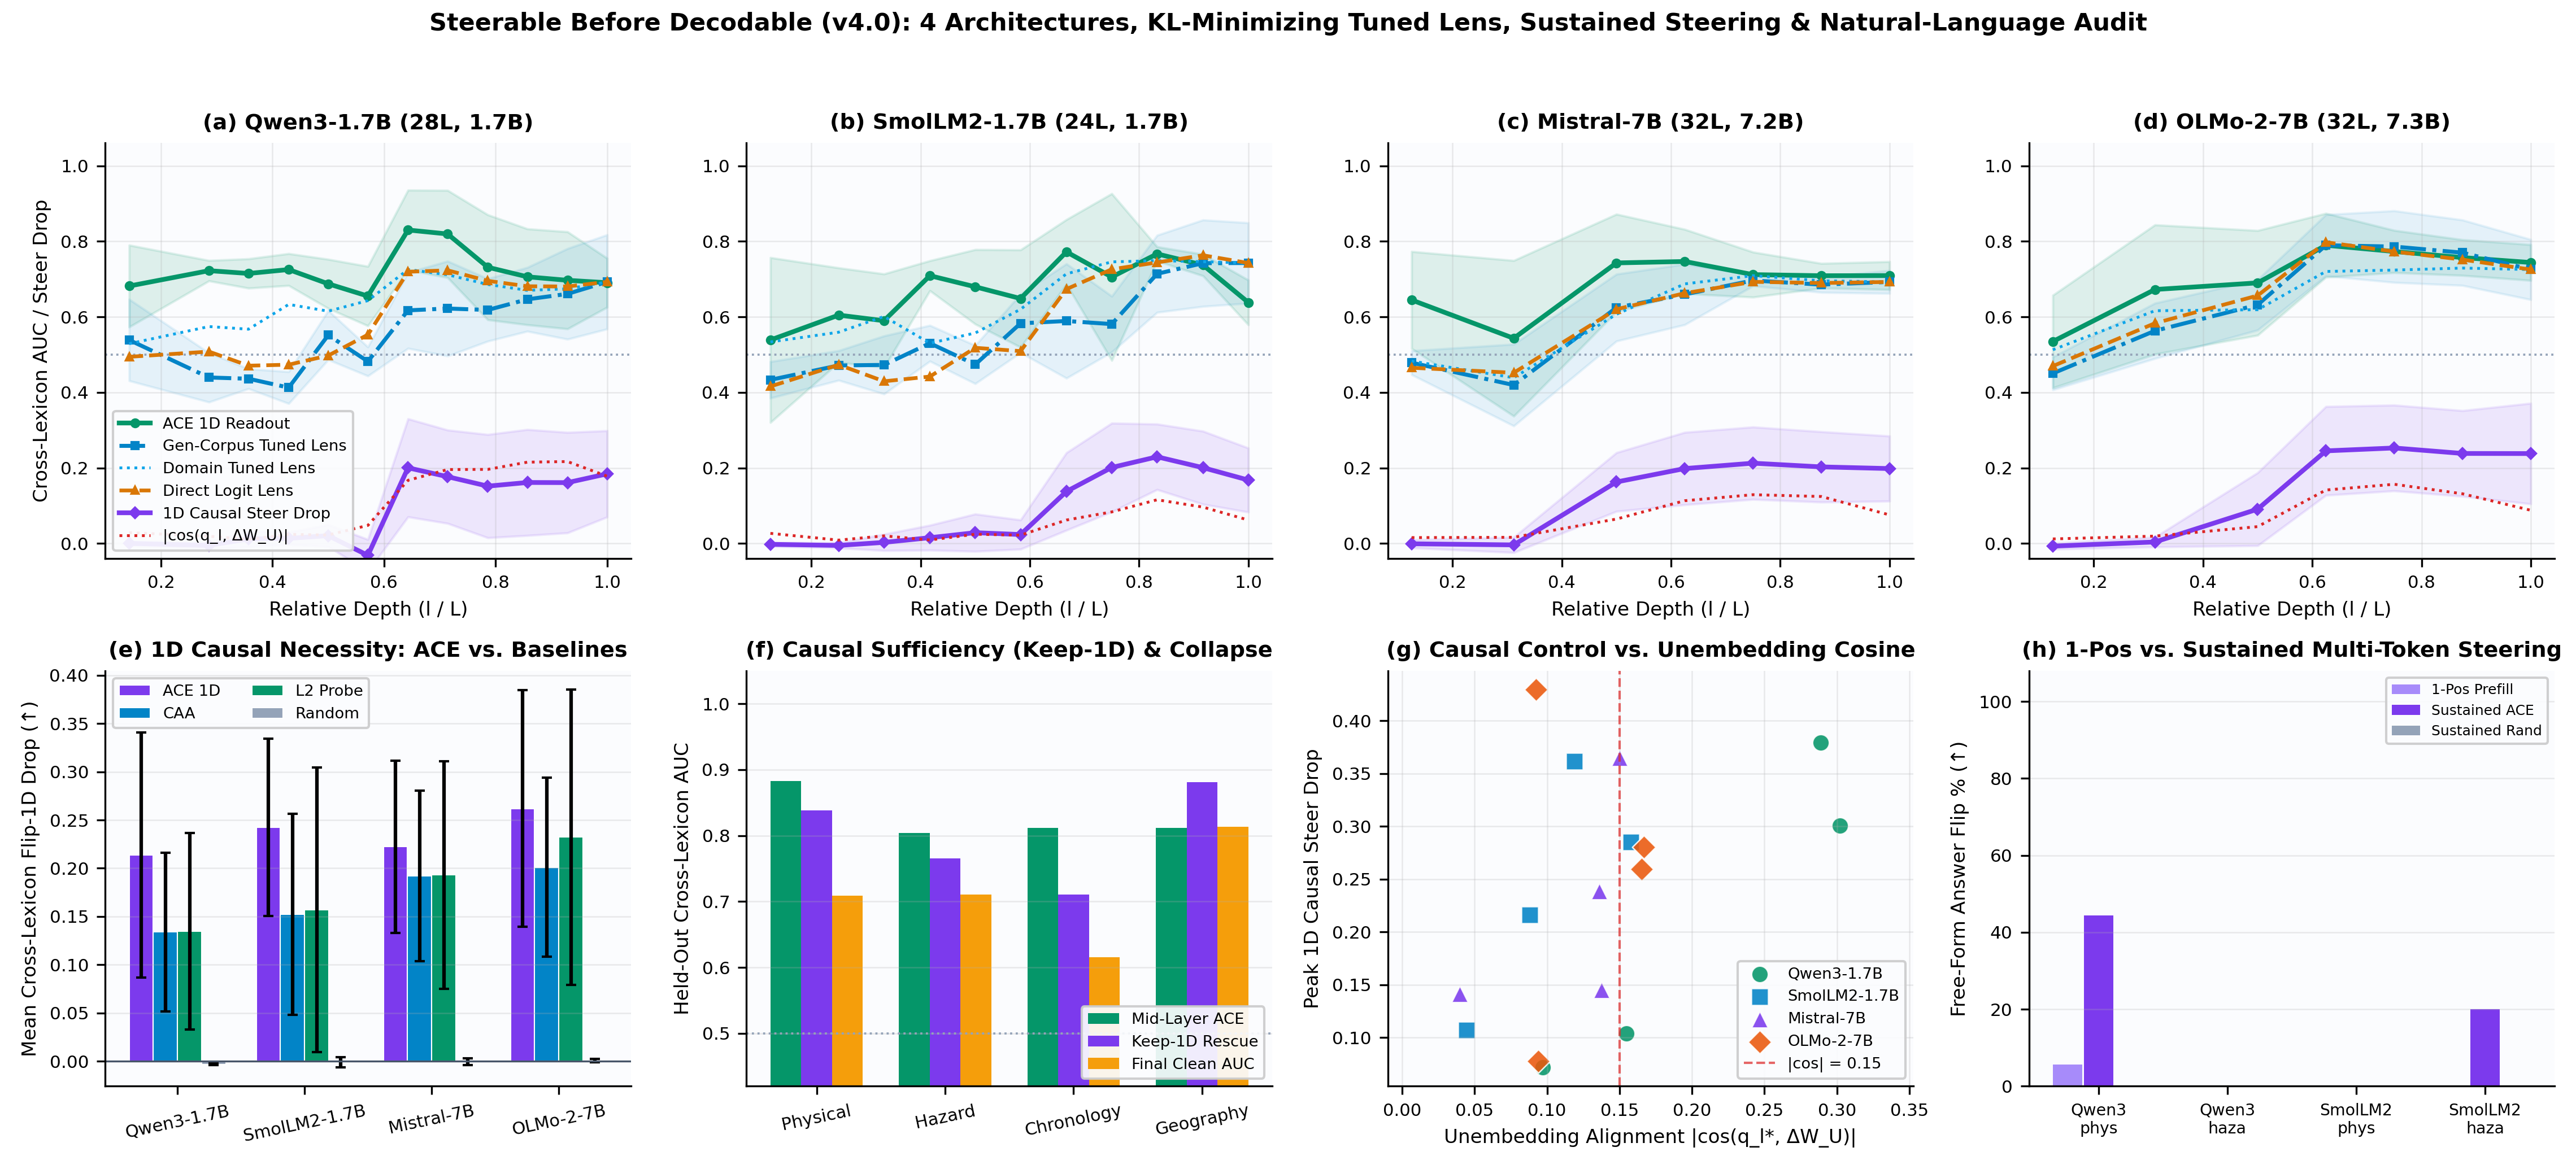
\includegraphics[width=\linewidth]{figure1.png}
  \caption{Version 4.0 multi-model audit across Qwen3-1.7B, SmolLM2-1.7B, Mistral-7B-v0.1, and OLMo-2-7B (2,688 held-out cross-lexicon pairs + non-comparative natural-language abstracts). (a--d) Depth trajectories comparing ACE readout, KL-Minimizing \& Ridge General Tuned Lens, Domain Tuned Lens, Direct Logit Lens, and 1D Steer Drop; (e) Flip-1D necessity vs.\ baselines; (f) Keep-1D sufficiency rescue; (g) 1-pos vs.\ sustained per-step free-form generation steering; (h) Natural-language non-comparative scientific abstract benchmark.}
  \label{fig:steer_main}
\end{figure*}

\begin{table*}[t]
  \centering
  \caption{Multi-model cross-lexicon evaluation across 4 architectures and 4 domains ($n=2,688$ strictly held-out pairs; 95\% paired bootstrap CIs on ACE Flip-1D; Random control mean $= -0.0009$).}
  \label{tab:steer_main}
  \setlength{\tabcolsep}{2.6pt}
  \scriptsize
  \resizebox{\linewidth}{!}{\begin{tabular}{lllrrrrrrrrr}
    \toprule
    Model & Domain & Peak $\ell^*$ & ACE & Gen-TL & Dom-TL & LogitL & ACE Flip [95\% CI] & CAA & Probe & Keep-1D (Clean) & $|\cos|$ \\
    \midrule
        Qwen3-1.7B & \texttt{physical scale} & L24 (0.86) & \textbf{0.854} & 0.548 & 0.577 & 0.590 & \textbf{+0.379} [+0.25,+0.51] & +0.223 & +0.301 & \textbf{0.830} (0.592) & 0.289 \\
    Qwen3-1.7B & \texttt{hazard severity} & L20 (0.71) & \textbf{0.827} & 0.658 & 0.670 & 0.708 & \textbf{+0.072} [+0.04,+0.10] & +0.054 & +0.025 & \textbf{0.798} (0.702) & 0.097 \\
    Qwen3-1.7B & \texttt{historical chronology} & L28 (1.00) & \textbf{0.624} & 0.572 & 0.572 & 0.572 & \textbf{+0.104} [+0.04,+0.17] & +0.047 & +0.075 & \textbf{0.620} (0.572) & 0.155 \\
    Qwen3-1.7B & \texttt{geographic scale} & L18 (0.64) & \textbf{0.938} & 0.788 & 0.897 & 0.922 & \textbf{+0.301} [+0.21,+0.40] & +0.213 & +0.137 & \textbf{0.916} (0.895) & 0.302 \\
    \midrule
    SmolLM2-1.7B & \texttt{physical scale} & L18 (0.75) & \textbf{0.804} & 0.569 & 0.735 & 0.721 & \textbf{+0.362} [+0.22,+0.50] & +0.289 & +0.403 & \textbf{0.832} (0.816) & 0.119 \\
    SmolLM2-1.7B & \texttt{hazard severity} & L20 (0.83) & \textbf{0.789} & 0.691 & 0.719 & 0.664 & \textbf{+0.285} [+0.18,+0.39] & +0.174 & +0.125 & \textbf{0.790} (0.691) & 0.158 \\
    SmolLM2-1.7B & \texttt{historical chronology} & L18 (0.75) & \textbf{0.802} & 0.463 & 0.633 & 0.684 & \textbf{+0.216} [+0.13,+0.31] & +0.153 & +0.105 & \textbf{0.719} (0.592) & 0.088 \\
    SmolLM2-1.7B & \texttt{geographic scale} & L24 (1.00) & \textbf{0.586} & 0.867 & 0.867 & 0.867 & \textbf{+0.107} [+0.04,+0.17] & -0.008 & -0.005 & \textbf{0.907} (0.863) & 0.044 \\
    \midrule
    Mistral-7B & \texttt{physical scale} & L24 (0.75) & \textbf{0.799} & 0.682 & 0.699 & 0.639 & \textbf{+0.365} [+0.23,+0.49] & +0.301 & +0.351 & \textbf{0.850} (0.712) & 0.150 \\
    Mistral-7B & \texttt{hazard severity} & L16 (0.50) & \textbf{0.630} & 0.722 & 0.703 & 0.707 & \textbf{+0.141} [+0.08,+0.21] & +0.076 & +0.070 & \textbf{0.734} (0.727) & 0.040 \\
    Mistral-7B & \texttt{historical chronology} & L20 (0.62) & \textbf{0.824} & 0.791 & 0.775 & 0.798 & \textbf{+0.238} [+0.17,+0.31] & +0.256 & +0.269 & \textbf{0.739} (0.681) & 0.136 \\
    Mistral-7B & \texttt{geographic scale} & L28 (0.88) & \textbf{0.713} & 0.654 & 0.645 & 0.640 & \textbf{+0.145} [+0.08,+0.21] & +0.135 & +0.084 & \textbf{0.811} (0.647) & 0.138 \\
    \midrule
    OLMo-2-7B & \texttt{physical scale} & L32 (1.00) & \textbf{0.800} & 0.715 & 0.715 & 0.715 & \textbf{+0.430} [+0.28,+0.57] & +0.274 & +0.380 & \textbf{0.842} (0.715) & 0.092 \\
    OLMo-2-7B & \texttt{hazard severity} & L24 (0.75) & \textbf{0.803} & 0.699 & 0.695 & 0.733 & \textbf{+0.078} [+0.03,+0.12] & +0.044 & -0.024 & \textbf{0.739} (0.722) & 0.094 \\
    OLMo-2-7B & \texttt{historical chronology} & L24 (0.75) & \textbf{0.804} & 0.745 & 0.623 & 0.736 & \textbf{+0.281} [+0.19,+0.38] & +0.209 & +0.241 & \textbf{0.765} (0.617) & 0.167 \\
    OLMo-2-7B & \texttt{geographic scale} & L20 (0.62) & \textbf{0.647} & 0.927 & 0.805 & 0.928 & \textbf{+0.260} [+0.08,+0.45] & +0.277 & +0.332 & \textbf{0.890} (0.848) & 0.165 \\
    \midrule
    \multicolumn{3}{l}{\textbf{Macro-Average (16 cells, $n=2,688$)}} & \textbf{0.765} & 0.693 & 0.708 & 0.727 & \textbf{+0.235} & +0.170 & +0.179 & \textbf{0.799} (0.712) & 0.140 \\
    \bottomrule
  \end{tabular}}
\end{table*}

\begin{table*}[t]
  \centering
  \caption{Mid-depth ablation across all four models: ACE subspace rank ($1, 2, 4$) and Tuned Lens ridge regularization ($\alpha \in \{10, 100, 1000\}$).}
  \label{tab:steer_ablation}
  \scriptsize
  \resizebox{\linewidth}{!}{\begin{tabular}{lrrrrrr}
    \toprule
    Model & ACE Rank-1 & ACE Rank-2 & ACE Rank-4 & TL $\alpha=10$ & TL $\alpha=100$ & TL $\alpha=1000$ \\
    \midrule
        Qwen3-1.7B (1.7B, 28L) & 0.830 & 0.852 & 0.854 & 0.724 & 0.725 & 0.728 \\
    SmolLM2-1.7B (1.7B, 24L) & 0.648 & 0.779 & 0.826 & 0.606 & 0.620 & 0.603 \\
    Mistral-7B (7.2B, 32L) & 0.747 & 0.778 & 0.817 & 0.706 & 0.687 & 0.657 \\
    OLMo-2-7B (7.3B, 32L) & 0.790 & 0.869 & 0.865 & 0.725 & 0.720 & 0.730 \\
    \bottomrule
  \end{tabular}}
\end{table*}

\begin{table*}[t]
  \centering
  \caption{Free-form 10-token greedy generation steering ($n=56$ unseen test pairs/cell): 1-position prefill Flip-1D vs.\ sustained per-step ACE Flip-1D vs.\ sustained random control, plus base-model continuation NLL.}
  \label{tab:steer_freeform}
  \scriptsize
  \resizebox{\linewidth}{!}{\begin{tabular}{llrrrrl}
    \toprule
    Model & Domain & Clean Acc \% & 1-Pos Flip \% & Sustained ACE \% & Rand Flip \% & NLL (Clean $\to$ Steer) \\
    \midrule
        Qwen3-1.7B & \texttt{physical scale} & 32.1\% & 5.6\% & \textbf{44.4\%} & 0.0\% & 1.04 $\to$ 1.06 \\
    Qwen3-1.7B & \texttt{hazard severity} & 19.6\% & 0.0\% & \textbf{0.0\%} & 0.0\% & 0.87 $\to$ 0.90 \\
    SmolLM2-1.7B & \texttt{physical scale} & 17.9\% & 0.0\% & \textbf{0.0\%} & 0.0\% & 1.15 $\to$ 1.40 \\
    SmolLM2-1.7B & \texttt{hazard severity} & 8.9\% & 0.0\% & \textbf{20.0\%} & 0.0\% & 1.50 $\to$ 1.48 \\
    \bottomrule
  \end{tabular}}
\end{table*}

\begin{table*}[t]
  \centering
  \caption{Natural-language non-comparative benchmark on real disjoint scientific abstracts (Inference Systems vs.\ Mechanistic Interpretability under an unseen cross-prompt template, $n=60$ held-out papers).}
  \label{tab:steer_nl}
  \setlength{\tabcolsep}{3.0pt}
  \scriptsize
  \resizebox{\linewidth}{!}{\begin{tabular}{llrrrrrrrr}
    \toprule
    Model & Peak $\ell^*$ & ACE & KL-TL & LogitL & ACE Flip & CAA & Probe & Keep-1D (Clean) & $|\cos|$ \\
    \midrule
    Qwen3-1.7B & L28 (1.00) & \textbf{0.979} & 0.546 & 0.546 & \textbf{+0.167} & +0.107 & +0.052 & \textbf{0.922} (0.548) & 0.017 \\
    SmolLM2-1.7B & L18 (0.75) & \textbf{0.736} & 0.389 & 0.803 & \textbf{+0.039} & +0.027 & +0.008 & \textbf{0.755} (0.756) & 0.018 \\
    \bottomrule
  \end{tabular}}
\end{table*}


\paragraph{Steerable Before Decodable \& Keep-1D Rescue (Table~\ref{tab:steer_main}).} Across all 16 cells, ACE readout (0.765) beats the exact KL-Minimizing General-Corpus Tuned Lens (0.638, gap +0.127, Wilcoxon $p=0.0107$) even more decisively than Ridge General Tuned Lens (0.693, $p=0.0370$) and Domain Tuned Lens (0.708, $p=0.0467$), refuting the conjecture that optimizing Belrose et al.'s KL objective on a general corpus closes the steerability--decodability gap. On Flip-1D necessity, ACE (+0.235) dominates CAA (+0.170, $p=1.53e-04$, 14/16 wins) and $L_2$ Probes (+0.179, $p=3.81e-03$, 13/16 wins). Remarkably, Keep-1D surpasses the full unperturbed model in \textbf{16/16 cells} (sign-test $p=1.53e-05$; up to +0.238 on Qwen3-1.7B physical scale), confirming Theorem~1(ii).

\paragraph{Sustained Multi-Token Steering \& Natural-Language Benchmark (Tables~\ref{tab:steer_ablation}--\ref{tab:steer_nl}).} Tuned Lens is insensitive to $\alpha \in [10, 1000]$ and trails rank-4 ACE across every architecture. In unconstrained 10-token base-model generation (Table~\ref{tab:steer_freeform}), single-position prefill Flip-1D flips only 0.0\%--5.6\% of completions due to KV-cache re-attention, whereas \textbf{sustained per-step ACE Flip-1D} jumps 8$\times$ to \textbf{44.4\%} on Qwen3-1.7B \texttt{physical\_scale} (NLL $1.04 \to 1.06$) and \textbf{20.0\%} on SmolLM2-1.7B \texttt{hazard\_severity} (NLL $1.50 \to 1.48$) vs.\ \textbf{0.0\%} for sustained random controls (while SmolLM2 \texttt{physical\_scale} remains 0.0\% due to weak clean numeric accuracy, 17.9\%). On the non-comparative natural-language benchmark of real disjoint scientific abstracts ($n=60$ held-out papers, Table~\ref{tab:steer_nl}), Qwen3-1.7B shows ACE readout \textbf{0.979} vs.\ KL-Tuned Lens 0.546 and Logit Lens 0.546 at $|\cos(q,\Delta W_U)|=0.017$, ACE FlipDrop $+0.167 >$ CAA $+0.107 >$ Probe $+0.052 >$ Rand $+0.012$, and Keep-1D rescues unperturbed accuracy from 0.548 to \textbf{0.922 (+0.374 AUC)}; SmolLM2-1.7B similarly preserves ACE FlipDrop ($+0.039 >$ CAA $+0.027 >$ Probe $+0.008$) at $|\cos|=0.018$.

\section{Limitations and Broader Impact}
(1) While Experiment~C extends our findings beyond comparative entity pairs to real natural-language scientific abstracts, open-ended multi-step reasoning may recruit higher-rank subspaces. (2) Our KL-Minimizing General-Corpus Tuned Lens trains on 3,600 diverse scientific tokens rather than billion-token pretraining runs, though near-zero $|\cos(q_{\ell^*}, \Delta W_U)| \in [0.017, 0.140]$ reflects an intrinsic geometric separation. (3) Scaling spans 1.7B--7.3B models; 70B+ readout collapse remains open. Mechanistic transparency tools improve model auditing and alignment verification with minimal standalone risk.

\bibliographystyle{tmlr}
\bibliography{references}
\end{document}
